\label{sec:experiments}

\subsection{Experiments with synthetic data}

This section presents results of the comparison of the proposed algorithm of change point detection (referred as \textit{LRTOnline} or \textit{LRTOffline}) with two other methods: \textit{Bayesian online changepoint detection (BOCPD)}  \citet{BayesOnlineWeb} and \textit{cpt.meanvar(PELT,$\ldots$)} (RMeanVar) from \citet{RPackage}. 
The first method is constructed for online inference, but so far as it returns CP location with each CP signal, it is also applicable for offline testing scenario. The idea of this method is predictive filtering: its forecasts a new data point using only the information have been observed already, where the distribution family is fixed (Normal for the tests in this paper). Bayesian inference calculates the length of the observed data (from the last CP).
The second algorithm also uses preliminary specified model. Its design focuses into finding multiple changes in mean and variance in Normally (another distributions also supported) distributed data. The returned set of change points is the result of sequential testing $H_0$ (existing number of change points) against $H_1$ (one extra change point) applying the likelihood ratio statistic of the whole data coupled with the penalty for CP count. Originally the method has offline change point detection interface, but one could adapt it for online case by buffering incoming data elements and clearing the buffer when at least one CP have been observed in the buffered data. 
In total, each of these two algorithms has modification in the way that allows one to use it in both online and offline testing mode. 

LRTOffline configuration:  \\
window sizes $(h_1, \ldots, h_W) = (10, 20, 40, 70)$; 
confidence for the upper bound of convolution with pattern $= 0.1$; 
window weights $(u_1, \ldots, u_W)  = (1.0, 2.0, 0.5, 0.2)$. 

LRTOnline configuration:  \\
window sizes $(h_1, \ldots, h_W) = (30, 50, 70)$; 
confidence $= 0.1$.


Quality of measurements  uses three following metrics: Normalised Mutual Information (NMI), Delay (average time interval in which CP have been detected after it had taken place), Precision  and Recall. The next equation defines 
NMI measure of two partitions ($X$, $Y$) of time range by change points
\[
\text{NMI}(X,Y) = 2 \frac{H(X) + H(Y) - H(X,Y)}{H(X) + H(Y)}.
\]
Higher NMI values (they are in $[0,1]$) correspond to better quality. 
Quality comparison in offline case apply NMI measure, while  for online mode involves Delay, Precision  and Recall. 

Synthetic test data have been generated for different values of difference norm of the data distribution parameter. Such values are denoted as \textit{delta}. Each delta corresponds to 10 sampled data sequences over which one compute measure average.  In online mode each data sequence could have one or none change points,  in offline mode -- two, one or none change points.       

\begin{figure}[ht!]
     \begin{center}
        \subfigure{%
            \label{fig:Precision_delta_N}
            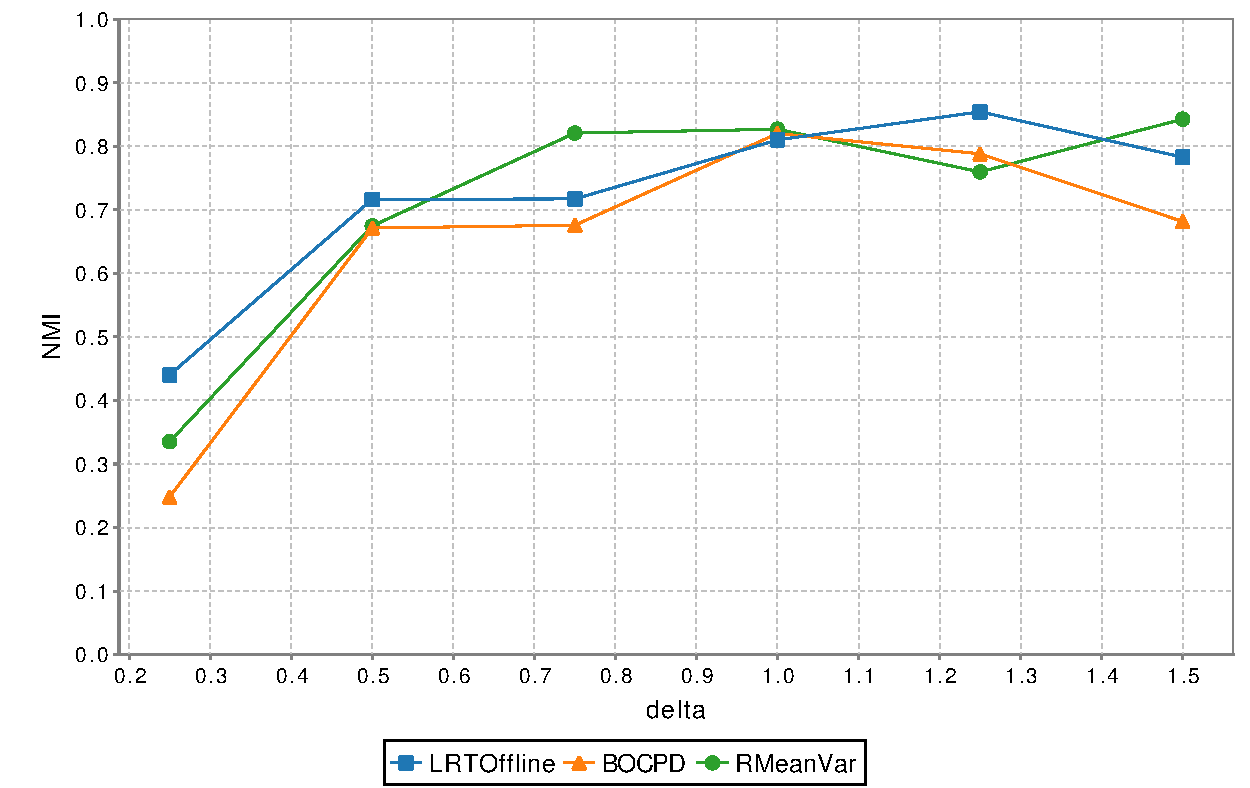
\includegraphics[width=0.4\textwidth]{images/NMI_delta_N}
        }%
        \subfigure{%
           \label{fig:Recall_delta_N}
           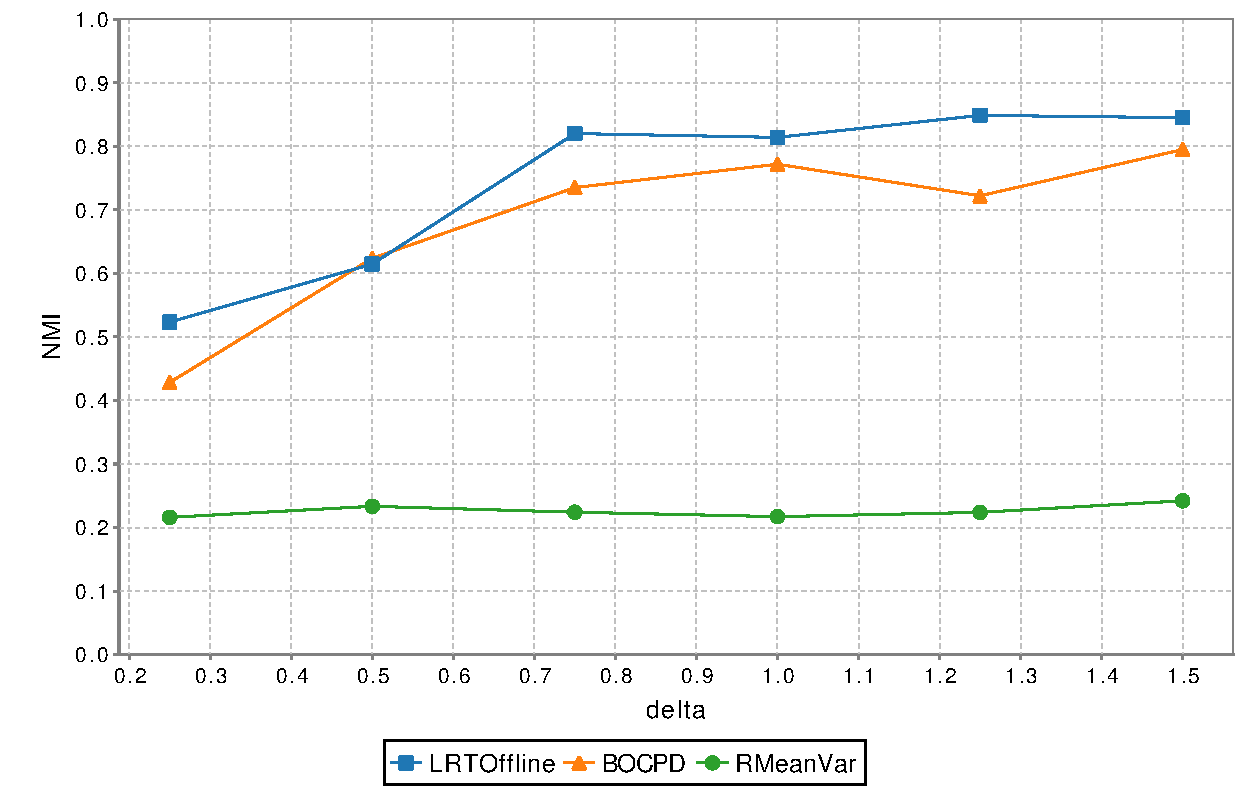
\includegraphics[width=0.4\textwidth]{images/NMI_delta_Po}
        }
         
         
%
    \end{center}
    \caption{%
        Offline mode. First data: $\ND(\theta(1), \theta(2))$, second data: $\Po(\theta)$,
        delta = $\Vert \theta_{12}^{*} \Vert$, data size = 340, PA for all methods is $\ND(\theta(1), \theta(2))$, NMI -- Normalized Mutual Information between predicted and reference partitions of time interval with change points, tests per delta = 10, change point per test = $\{0,1,2\}$.
     }%
   \label{fig:subfigures}
\end{figure}


\begin{figure}[ht!]
     \begin{center}
        \subfigure{%
            \label{fig:Precision_delta_N}
            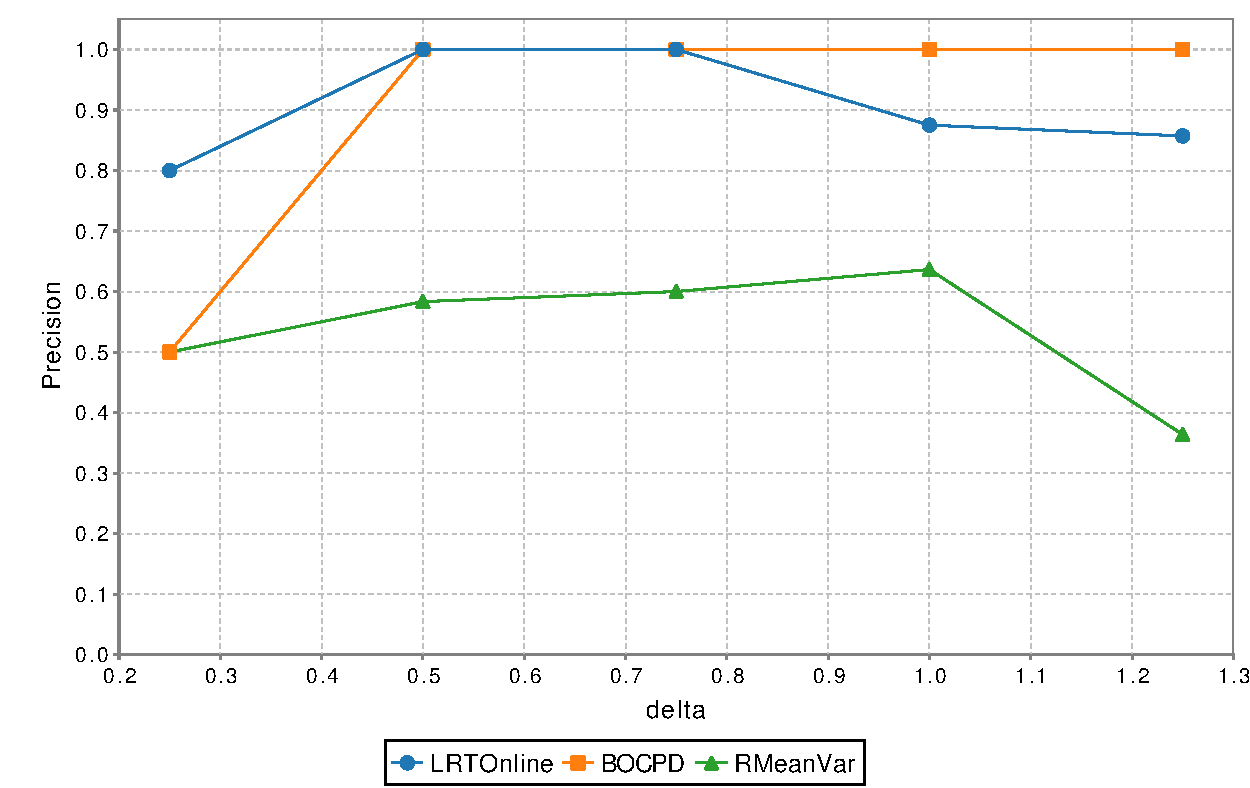
\includegraphics[width=0.3\textwidth]{images/Precision_delta_N}
        }%
        \subfigure{%
           \label{fig:Recall_delta_N}
           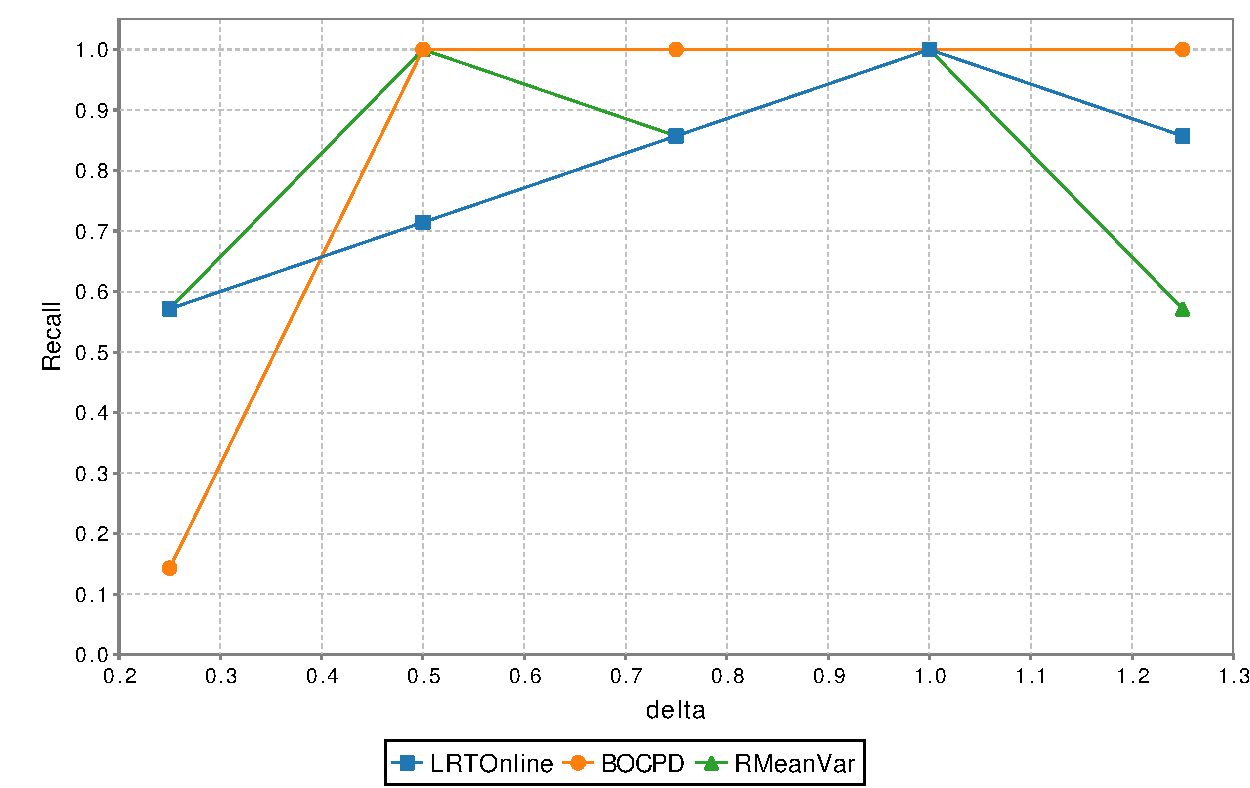
\includegraphics[width=0.3\textwidth]{images/Recall_delta_N}
        }
         \subfigure{%
           \label{fig:Delay_delta_N}
           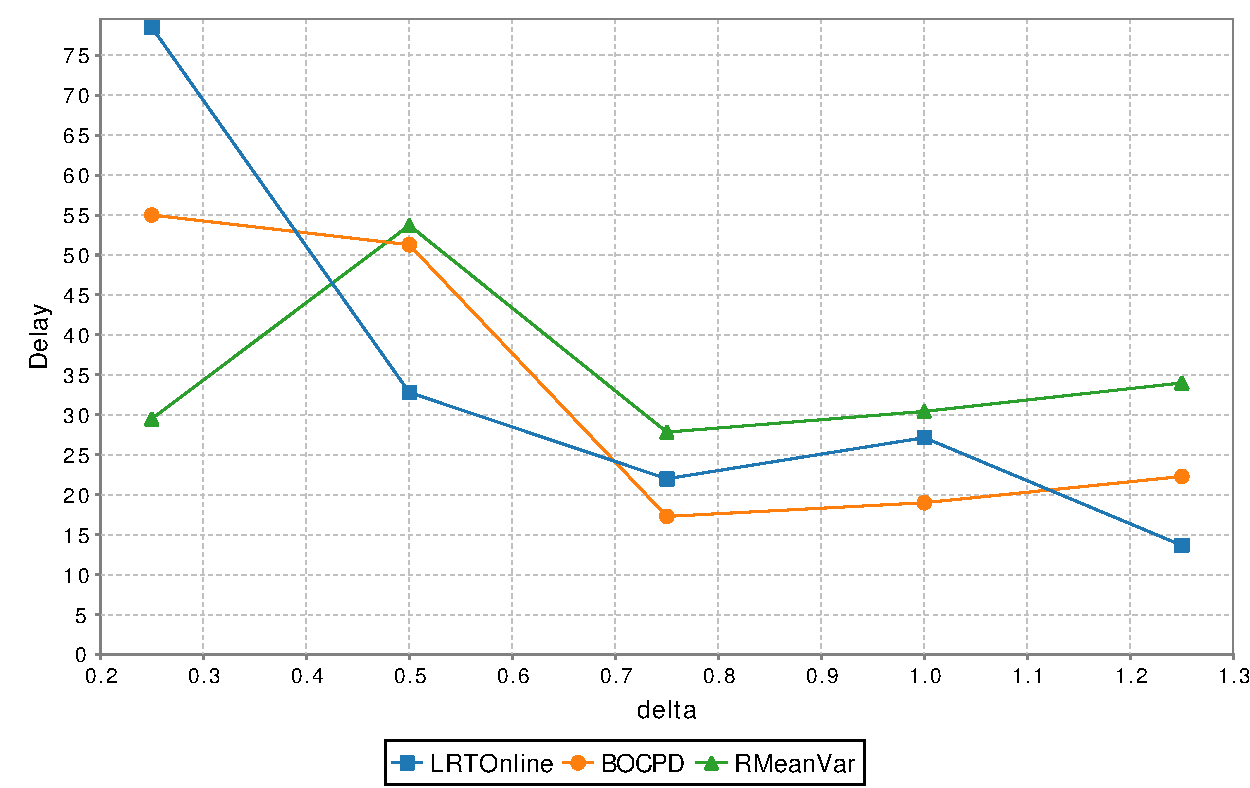
\includegraphics[width=0.3\textwidth]{images/Delay_delta_N}
        }\\%  ------- End of the first row ----------------------%
          \subfigure{%
            \label{fig:Precision_delta_N}
            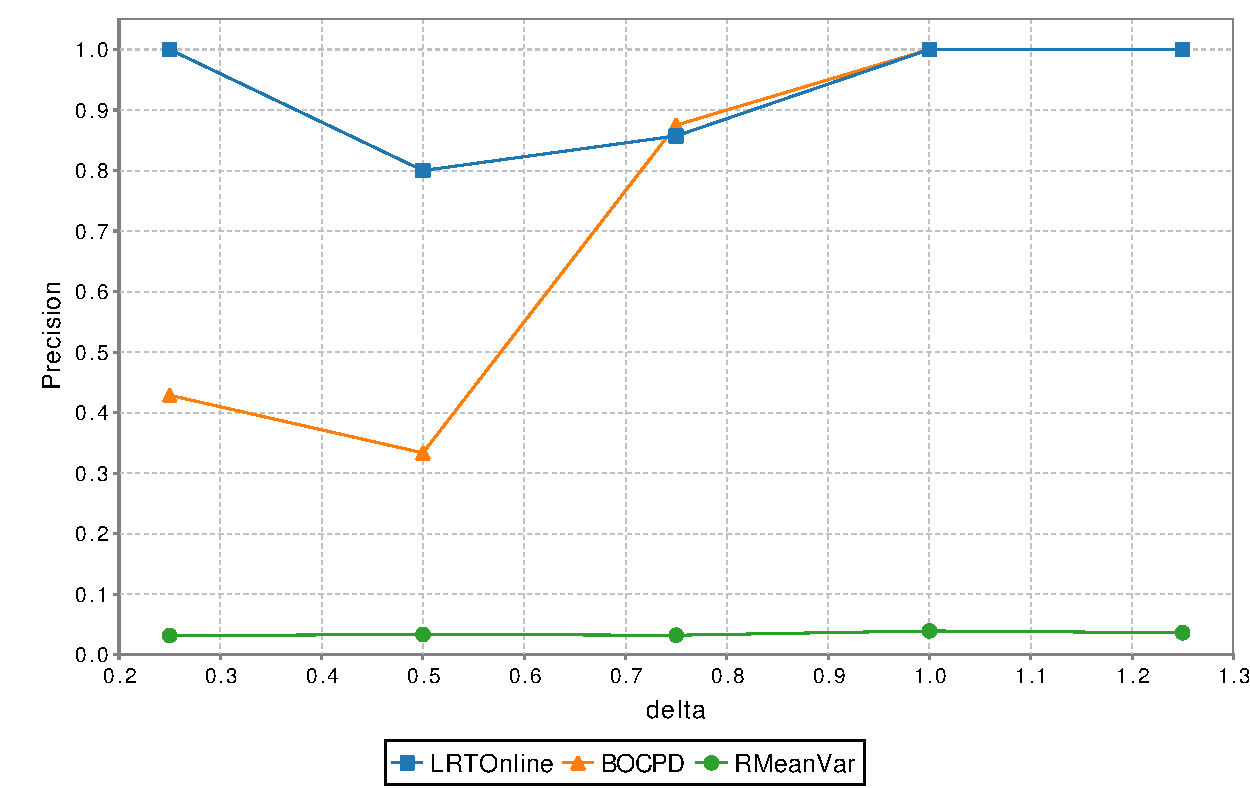
\includegraphics[width=0.3\textwidth]{images/Precision_delta_Po}
        }%
        \subfigure{%
           \label{fig:Recall_delta_N}
           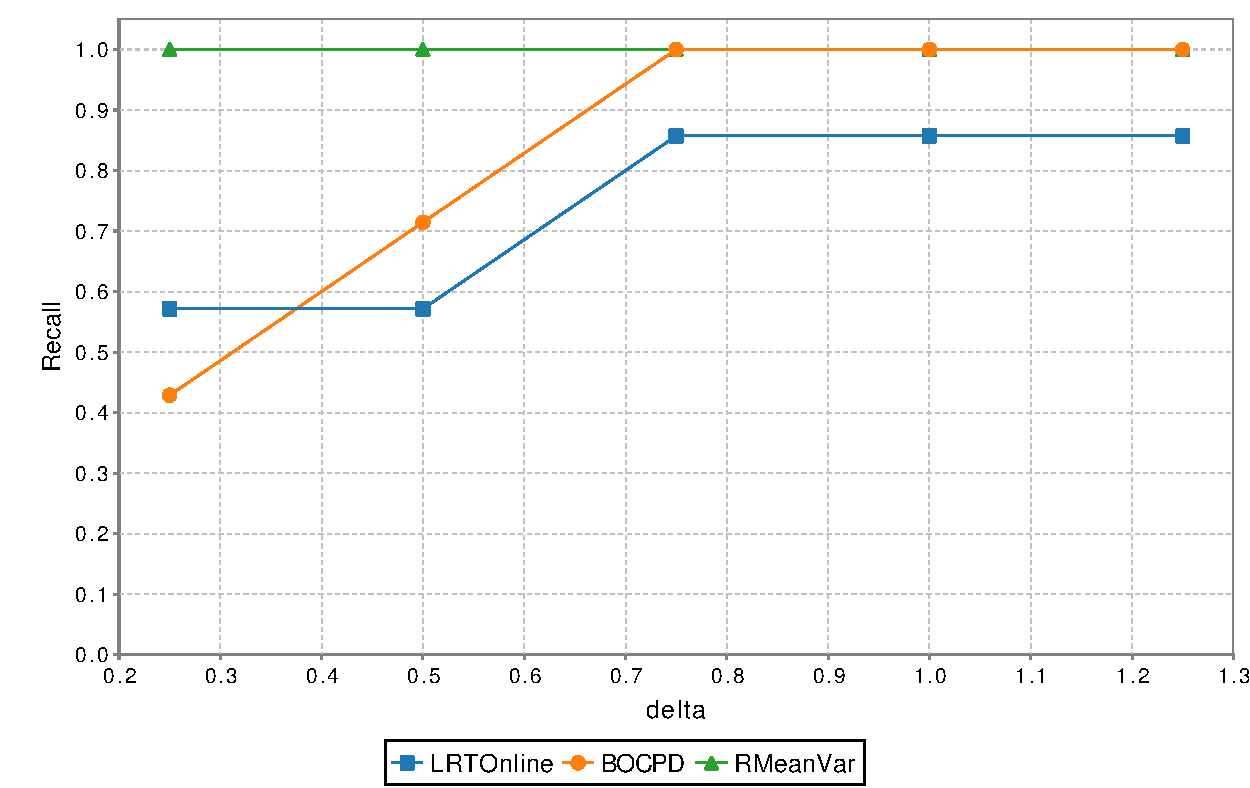
\includegraphics[width=0.3\textwidth]{images/Recall_delta_Po}
        }
         \subfigure{%
           \label{fig:Delay_delta_N}
           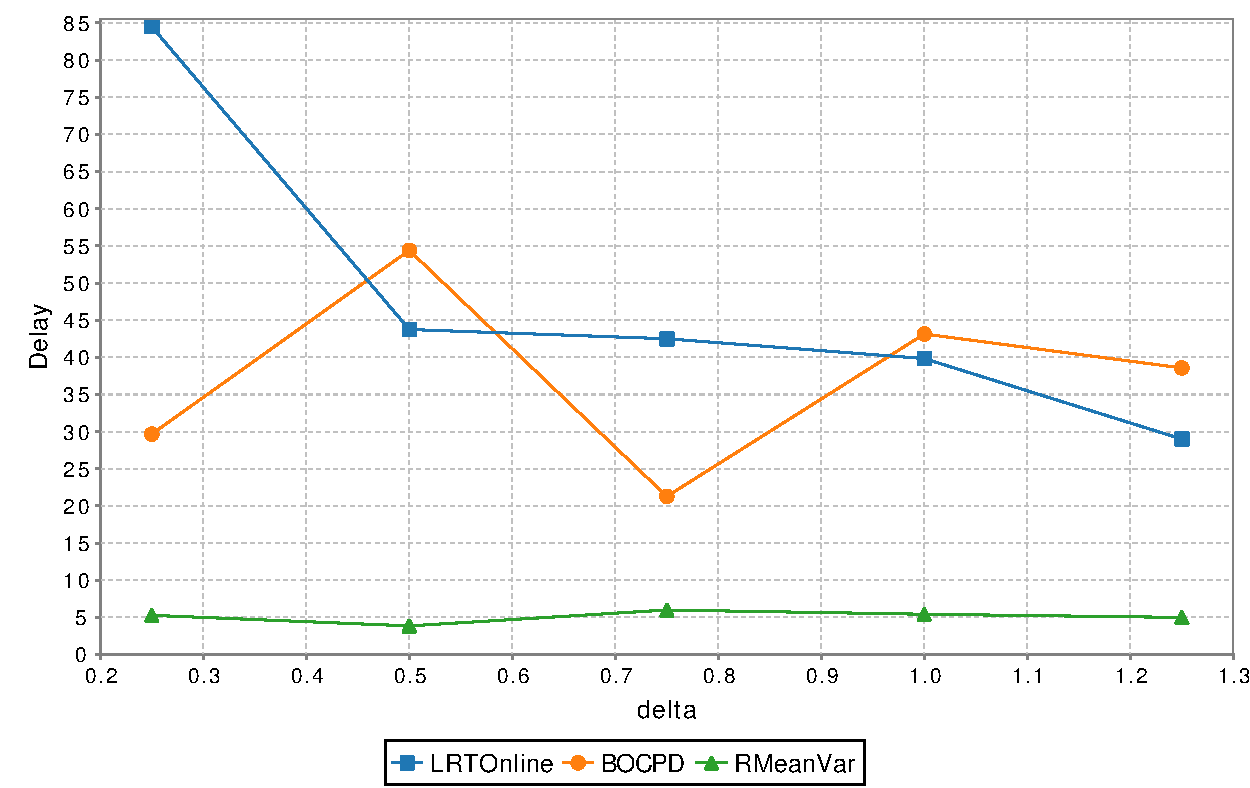
\includegraphics[width=0.3\textwidth]{images/Delay_delta_Po}
        }
%
    \end{center}
    \caption{%
       Online mode. First row data: $\ND(\theta(1), \theta(2))$, second row data: $\Po(\theta)$,
        delta = $\Vert \theta_{12}^{*} \Vert$, data size = 340, PA for all methods is $\ND(\theta(1), \theta(2))$, tests per delta = 10, change point per test = $\{0,1\}$.
     }%
   \label{fig:subfigures}
\end{figure}

In the offline tests with Normal data all the methods achieves similar NMI scores, nonetheless LRTOffline is more stable for decreasing strength of CP (delta). In the tests with Poisson data (misspecification) RMeanVar has relatively low quality. The online tests characterizes the proposed method (LRTOnline) as more stable along different delta values what is accomplished by multiscale heuristic.      

 The experiments reveal following meaningful properties of the proposed method configuration:

\begin{enumerate}
\item Quality is sensitive to selection of interval for upper bound calibration of convolution in offline mode. For example in data $\ND(0,1)$.sample(100) $\cup$ $\ND(1,2)$.sample(100) is preferable to use only slice of 0 to 100 elements for calibration, because of lower $\Var \dxi$.  Generally one should find change points in $tr(B_1 + B_2)$ according to remark~\ref{dxi_limit} from Section \ref{sec:theory} and run calibration in the range with the lowest values of $tr(B_1 + B_2)$. This improvement additional  requires approximation of the convolution maximum in larger data ranges.   

\item It is influenced to find out the minimal $h$ sufficient for bootstrap usage. Small $h$  improves Delay but makes unable to keep high level of  Precision and Recall in online mode. 
\end{enumerate}

\subsection{Experiments with real data}

Here data from 1972-75 Dow Jones Returns  \citet{BayesOnlineWeb}  describes several major events with potential macroeconomic effects (the most significant among them are the Watergate affair and the OPEC oil embargo). 
Convolutions plot with its upper bounds on this dataset appeared to be a nice illustration of multiscale search importance: CP near $t=325$ is better 	
perceptible when window size is equal to 30 and CP near $t=600$ has more perceptible convolution when window size is equal to 70. Two plots presented below includes convolutions with Static and Fitted Patterns, where one could remark better separability of convolution peaks in fitted case.       
 

\begin{figure}[ht!]
     \begin{center}
        \subfigure{%
            \label{fig:Precision_delta_N}
            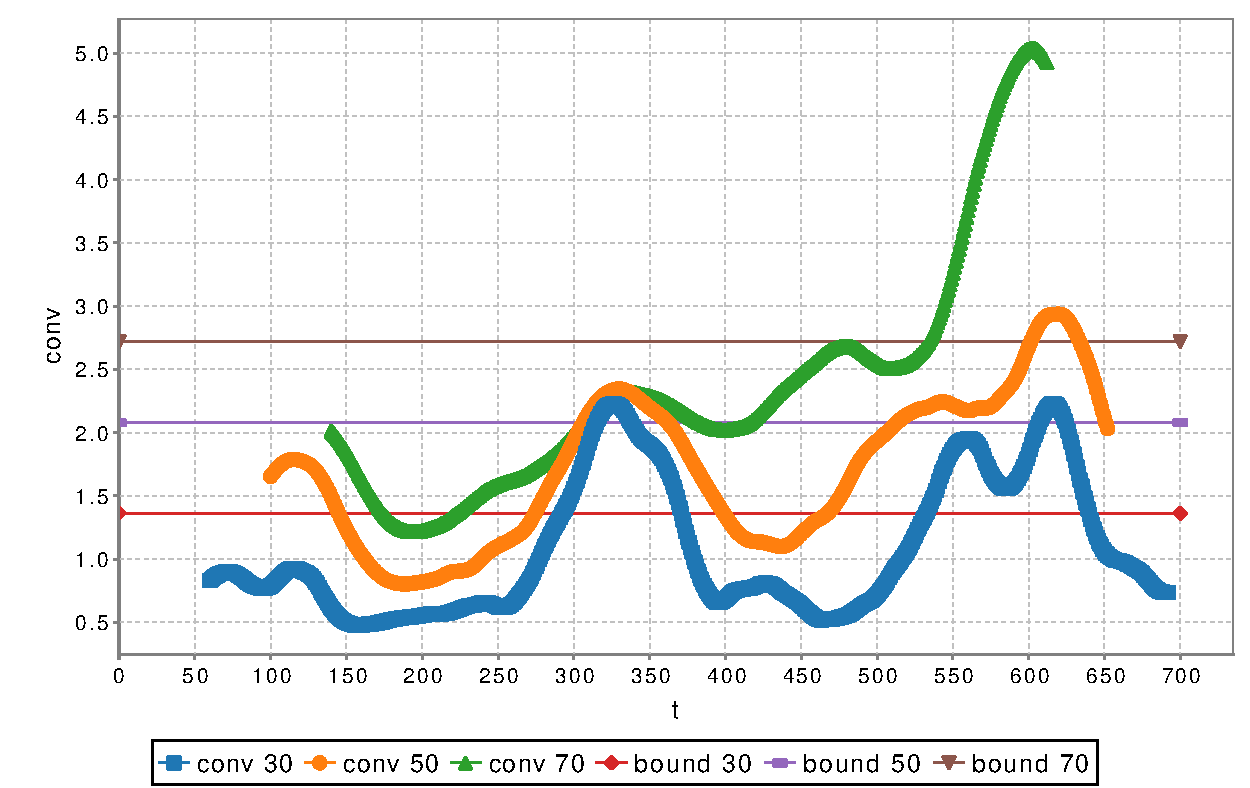
\includegraphics[width=0.45\textwidth]{images/watergate1.pdf}
        }%
        \subfigure{%
           \label{fig:Recall_delta_N}
           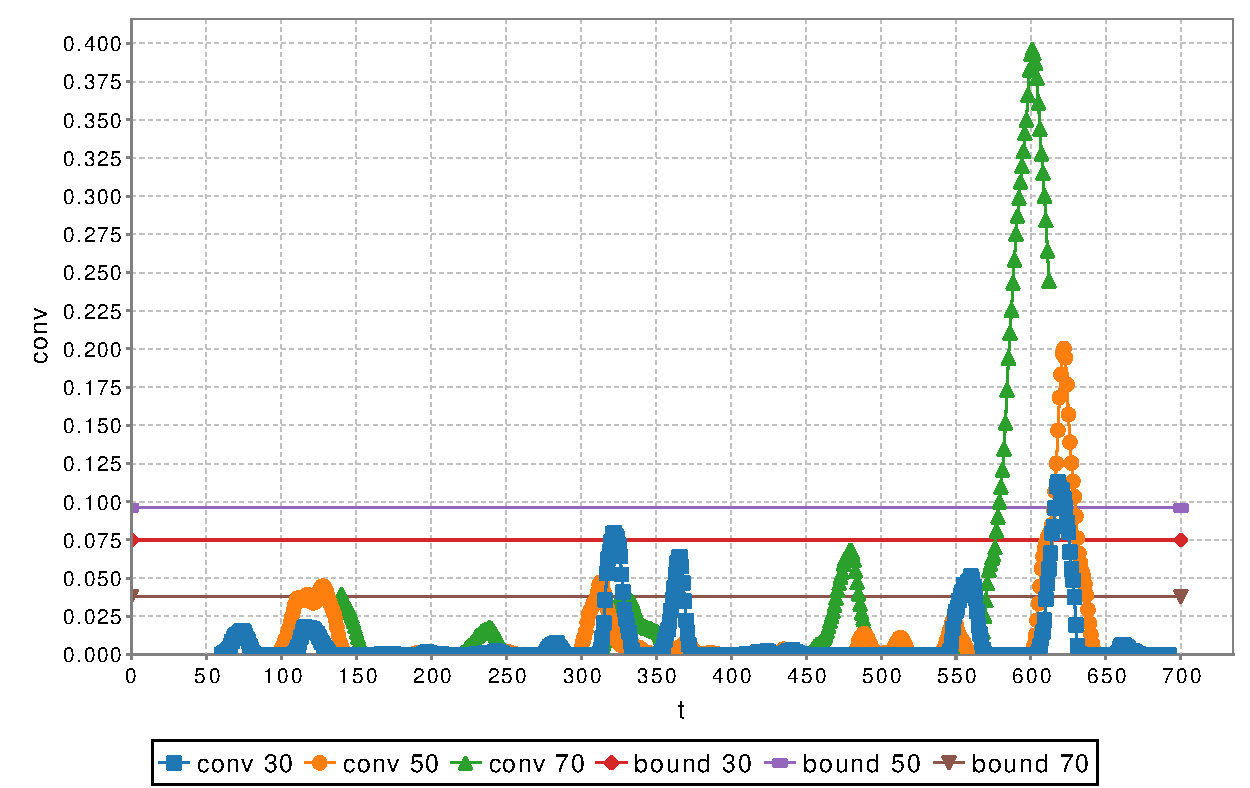
\includegraphics[width=0.45\textwidth]{images/watergate2.pdf}
        }
         
         
%
    \end{center}
    \caption{%
        Data: daily returns of the Dow Jones Industrial Average from July 3, 1972 to June 30, 1975.
        Left plot -- convolution with static triangle pattern; right plot -- convolution with fitted triangle pattern. The time axis is in business days, conv 30 (50, 70) corresponds to pattern with window size 30 (50, 70), bound 30 (50, 70) corresponds to convolution upper bound. Three reference CP are presented: the conviction of G. Gordon Liddy and James W. McCord, Jr. on January 30, 1973 ($t = 142$); the beginning of the OPEC embargo against the United States on October 19, 1973 ($t = 325$); the resignation of President Nixon on August 9, 1974 ($t = 548$).
     }%
   \label{fig:subfigures}
\end{figure}


\subsection{Sources}

Demo of the LRTOnline method is available by link  \\ https://localcpdetector.shinyapps.io/localCP

Scala project with LRTOffline and LRTOnline methods could be cloned from \\
https://github.com/nazarblch/cpd \\
which also includes testing system for abrupt change points detection applications and generated data used in the experiments. 





